\documentclass[UTF8]{ctexart} 
%\usepackage{homework}
\usepackage{geometry}
\geometry{a4paper,scale=0.8}
\usepackage[table,xcdraw]{xcolor}
\usepackage{graphicx} %插入图片的宏包
\usepackage{float} %设置图片浮动位置的宏包
\usepackage{subfigure} %插入多图时用子图显示的宏包
\usepackage{enumerate}
%\usepackage{fancyhdr}  % header,footer的设置
%\usepackage{extramarks}
\usepackage{amsmath}  % 数学公式
\usepackage{amsthm}
\usepackage{amsfonts}
\usepackage{tikz}  % 绘图
\usepackage{algorithm}  % 算法
\usepackage{algorithmicx}
\usepackage{algpseudocode}  % 伪代码
%\usepackage[UTF8]{ctex}  % 支持中文
%\title{我的份}
%\author{randow}
%\begin{document}
%\maketitle
\title{
	
\includegraphics[scale = 0.8]{HDU.png}\\
    \vspace{1in}
    \textmd{ \Huge\textbf{创业基础}}\\
    \textmd{\textbf{《“万品客”跨组织人才管理系统》}}\\
    \textmd{\textbf{商业计划书}}\\
   	\vspace{3in}
   	\large{小组 \qquad}\\
	\textmd{项目组成员:\qquad}\\
	\textmd{班级:\qquad}\\
	\textmd{指导老师:\qquad}\\
%    \normalsize\vspace{0.1in}\small{\hmwkCompleteTime }\\
%    \vspace{0.1in}\large{\textit{\hmwkClassInstructor\ }}\\
}
%\usepackage{enumerate}
%\author{\hmwkAuthorName \\ 
%	\hmwkAuthorStuID}
%\date{}

\begin{document}
\maketitle
\newpage
\tableofcontents
\newpage
\section{项目概要}
在人才招聘方面,中小微企业面临着招人难、留人难的问题。完成一个岗位的人才招聘,既包括:招募、甄选、录用、培训等显性成本;也包括:岗位空缺、员工离职、适应交接等隐性成本。相比大企业,中小微企业没有能力对应聘人员进行详尽的背调工作,只能采取简单地致电前雇主hr的方式。然而,碍于情面,前雇主hr并不会对员工做出评价,hr难以得到对应聘人员的正确回馈,招不到人、招工慢、招错人等问题增加了企业在招工方面的成本,甚至后续给企业造成损失。

当今时代,互联网飞速发展,在各行各业发挥巨大作用,极大改变了行业面貌。在中小企业招工方面也可依托互联网找到合适的解决方案,但现在还没有一套适用于中小微企业的员工信息查询系统。

中小微企业招工时的一大问题为无法得到应聘人员的有效信息,导致在是否聘用上无法抉择。建立一套跨组织人才管理系统,借助互联网的实时性、开放性与共享性,hr在招聘时能快速得知应聘人员情况。企业在系统上为雇员建立人才档案,记录员工工作状况和重大事件。招聘时可以轻松了解应聘人员在先前公司的工作情况,帮助中小微企业解决招工时的信息不足问题,完成员工招聘与背景调查工作,可以极大降低中小微企业在招工方面的成本,具有现实意义。

本项目致力于打造一款解决小微企业招聘问题的跨组织人才管理系统。使员工与职业有关的信息透明化,降低企业招聘成本;同时适用于求职人员投放简历,提高应聘效率的系统。
\section{可行性分析}
\subsection{项目优势与劣势}
\subsubsection{优势分析}
目前绝大企业招工都是采用传统的纸质简历+面试筛选模式,缺乏一个好的线上平台,对所有简历进行分析筛选,十分不高效,企业招聘市场也存在巨大的存量,线上HR平台的市场潜力是巨大的

对于企业内部人员的管理,我们也需要对不同员工的各项数据,各个部门的各项统计数据进行统计、分析和计算,采用线上平台能够大大提升统计的效率。
\subsubsection{劣势分析}
对于大公司来说(尤其是互联网公司),线上人才管理系统已经得到了广泛的适用,有可能会将其对公众开放,从而产生竞争。

人才的评价和评定是多方面多角度的,而且这对于不同的公司的需求也不相同,这会大大增加平台设计的复杂度。
\subsection{机遇分析}
近年来企业对人才的需求日益高涨。根据Michael Page(中国)发布《2021人才趋势报告》:技术、医疗保健与生命科学领域等领域对人才的需求日益增长,雇主也将继续争夺优质人才,我们的客户对远程招聘海外优质人才的需求量也在增加。

其次,灵活人才和临时工需求量增大。灵活用工的就业形势在某些亚太市场已经存在了数十年之久,但在部分亚洲市场,这种形式仍处于萌芽状态。报告指出,新冠疫情以及相关市场的不确定性加速了这一早存在的需求增长。

据普华永道发布的《未来的工作 – 通往2022年的旅程》,46\%的人力资源专业人士预计,到2022年所在企业的员工队伍中至少有20\%由灵活人才或者临时工组成。Michael Page在2018年开展的一项调查显示,中国96\%的职场人士有兴趣成为灵活人才,而75\%的在华企业透露他们曾雇佣过灵活人才。

报告指出,在充满不确定性和未知的未来,灵活人才和临时工可以带来企业所需的灵活性。这类招聘不受员工人数限制,可以解决项目用人需求、节约成本并提高用工灵活性。雇主只需根据候选人实际工作的小时/天数来支付费用。数据显示,26\%的企业会雇佣短期灵活人才弥补现有员工队伍中的技能缺口。

短期临时工人的招聘,会对HR造成格外的工作量,如果是进行线上统计和整理,整体的复杂度就下降了许多

对于职场人士来说,这种就业方式的高灵活性,让他们能够在短时间内获得多样化的经验、丰厚报酬和培养可转移的软技能。特别是在经济不景气时期,灵活用工或者基于项目的工作机会,对职场人来说也是增加了就业机会。另外,如果一名职场人在尝试了灵活人才服务方式后发现自己并不适合,再重新回到全职工作岗位也很容易


灵活的就业方式能够极大的促进招聘市场的活跃度,于此同时自新冠肺炎疫情爆发以来,全球经济环境充满不确定性,其引发的经济衰退对整个亚太地区也造成了打击。不少企业为控制成本,选择暂停或减少招聘新员工,中国大陆在2020年的招聘活动减少了30\%。国内招聘市场有巨大的潜力。
\subsection{竞争和挑战}
\subsubsection{市场认知尚未打开}
线上招聘平台在中国的发展起步较晚,除了互联网公司,绝大多数公司还需要提交纸质建立,并且进行线下面试,另一方面,相较于国外早已实现的一些在线HR平台来说,国内还存在一部分的纸质档案难以线上的问题。如果要实现线上人才管理,人才档案的电子化的推进还是有些许不足。
\subsubsection{开发线上系统设计到信息安全问题}
人才档案属于极度敏感的隐私数据,如果出错或者泄露,后果将不堪设想,关于网站信息安全方面的建设也是不可小觑的。

事实上,根据《档案管理违法违纪行为处分规定》(监察部、人力资源社会保障部、国家档案局令第30号)和《中共中央组织部关于进一步从严管理干部档案的通知》的有关要求:

如果擅自向外公布或泄露流动人员人事档案内容,将由党委组织部门和政府人力资源社会保障部门严肃查处,视情节轻重给予当事人和相关责任人批评教育或党纪、政纪处分;触犯法律的,要依法追究责任。
\subsubsection{大公司介入相对容易}
虽然目前已经有了一定的技术积累,但是大公司(腾讯、阿里等)在其他一些方面的技术积累雄厚,例如前端、框架技术、服务器处理能力的技术也不容小觑。
\section{市场分析}
\subsection{需求背景}
人才市场作为一种信息资源的集散地,求职者和用人单位要查询的资料繁多,包含很多的信息数据的管理。现今,有很多的人才市场都是初步开始使用,甚至尚未使用计算机进行信息管理。根据调查得知,他们以前对信息管理的主要方式是基于文本、表格等纸介质的手工处理,对求职者和用人单位的登记是采用手抄的方式进行的,数据信息处理工作量大,受个人的字迹影响容易出错;查询情况以及签约情况的统计和核实等往往采用人工统计的方法,准确率低;由于数据繁多,容易丢失,且不易查找。总的来说,缺乏系统,规范的信息管理手段。


尽管有的人才市场有计算机和大屏幕,但是尚未用于信息管理,没有发挥它的效力,资源闲置比较突出。数据处理手工操作,工作量大,出错率高,出错后不易更改。人才市场采取手工方式对用人单位和就业人员的登记情况进行人工管理,由于信息比较多,登记信息管理工作混乱而又复杂;一般登记情况是记录在当时的一张登记表上,根据登记表的大体内容分类存放,人才市场的工作,人员和管理员也只是当时对它比较清楚,时间一长,如再要进行查询,就得在众多的资料中翻阅、查找了,造成查询费时、费力。如要对很长时间以前的信息资料进行更改就更加困难了。基于这此问题,我认为有必要建立一个人才市场信息管理系统,使人才信息管理工作规范化,系统化,程序化,避免信息管理的随意性,提高信息处理的速度和准确性,能够及时、准确、有效的查询和修改已经记录的信息情况。

\subsection{制约因素}
\begin{itemize}
	\item[1)]
		企业对人力资源开发重视不高。区内大部分企业对人力资源的开发均未列入工作考核范围,缺乏对人力资源开发的整体规划,在人力资源的引进和教育培训、人才的管理和成长平台搭建、人才的人文关怀和薪酬体系的构建以及企业文化建设等方面,处于空白状态,如在培训方面,未将之作为提升业绩的基础,培训机制空白。部分企业缺乏人才储备与培养意识,没有把目光放远,引进高层次、高技术管理方面人才,也没有对现有人才进行挖掘和培养。
	\item[2)]
		企业对职业技能培训认识不足。由于企业规模小,培训场所、培训时间和培训经费难以保障,培训内容多以企业的应急需求为主。为了避免培训后员工流失而造成的培训投资风险,多数中小企业宁肯从市场上现招相关人人才也不愿花钱自行培养。部分用人单位为减少人员成本,仍继续招聘无职业资格证书人员就业上岗。这种重一般使用,轻挖掘、培养人才,人才依靠外部引进的人力计划,不仅增加了企业的成本,又打击了原有人才的积极性,也是造成中小企业人才流动频繁的重要原因之一。
	\item[3)]
		人力资源服务机构发展滞后。人力资源服务机构在才资源合理配置中发挥着越来越重要的作用。新区人力资源服务机构发展滞后,具体表现在: 一是公共人力资源服务机构人员配置不足,人员业务技能水平不高。二是民营人力资源中介机构层次不高。目前新区民营人力资源中介机构数量相对太少,服务形式不能充分满足需求,现有的公开登记的机构中既缺少私营的猎头公司,也缺少中外合资性质的人力资源中介组织。就服务形式而言,最多的是提供人才信息,提供档案保管等服务。高端的人力资源服务外包、猎头、管理、咨询等业务开展较少。
	\item[4)]
		政策的制定和落实缺乏衔接。政策制定和落实的衔接问题体现在以下几个方面: 一是有的政策与职能部门的工作之间缺乏衔接。有的政策在制定过程中没有充分听取政策执行部门的意见,在具体政策执行时遇到了障碍或困难。二是有的政策与现有人才的培养使用之间缺乏衔接。部分制定的优惠政策重在引进人才,忽视了现有人才的培养使用,挫伤了现有人才的工作积极性,造成人才的非正常流失。比如引进的硕士以上人才享受薪酬和购房补贴,现有人才没有相应补贴,产生待遇上的不平衡。三是现有人才政策申报流程繁琐,资金落实周期太长。
\end{itemize}

\subsection{需求分析}
\subsubsection{业务需求}
随着计算机技术,网络技术和信息技术的发展, 现在的办公系统更加趋于系统化,科学化和网络化,网络办公自动化系统是计算机技术和网络迅速发展的一个办公应用解决方案,它的的主要目的是实现信息的交流和信息共享,提供协同工作的手段,本系统对公司的人力资源进行管理,为人才管理人员提供一套简单的操作,使用可靠,界面友好,易于管理和使用的处理工具,对人才资源各种数据进行统一管理,避免数据存取,数据处理的重复, 提高工作效率,减少数据处理的复杂。
\subsubsection{用户需求}
跨组织人才管理系统在企业中起着通行桥梁的作用,通过与其它的各个管理系统模块的信息连接,将整个企业有机、高效地带动起来,使得企业各个方面的工作因人力资源管理系统的高效、简便而更加顺利。

企业方面: 可以有效进行对职工信息管理;增加、删除、修改员工信息;薪金发放;考勤以及招聘等工作。

职工方面:每个职工都可以对自己的信息进行查看,查询薪金发放情况以及职称评比情况。

\subsection{调查报告}
\subsubsection{企业跨组织人才管理系统使用意向调查表}
我们是一个大学生项目团队,正在设计与开发一款面向小微企业HR、在职员工、求职者的跨组织人才管理系统。在这个系统中,企业HR可进行员工的人事管理,员工跳槽去一家新公司时,这家用人单位将可查阅本系统内的人才档案,系统会对关键数据进行脱敏。该系统旨在为企业解决招聘中的背调难、成本高、不深入的问题。现在有以下问题需要您的意见,对我们的项目非常重要。
\begin{enumerate}[1.]
	\item 您的身份 [单选题] *
	\begin{enumerate}
		\item 企业HR (请跳至第2题)
		\item 在职员工 (请跳至第3题)
	\end{enumerate}
	\item 您所在的公司,是否有电子化的人事管理系统 [单选题] *
	\begin{enumerate}
		\item 有
		\item 没有
	\end{enumerate}
	\item 您所在的公司是否有电子化的人才管理系统 [单选题] *
	\begin{enumerate}
		\item 有
		\item 没有
	\end{enumerate}
	\item 那您是否期待公司使用一个跨组织人才管理系统进行管理 [单选题] *
	\begin{enumerate}
		\item 期待
		\item 不期待
	\end{enumerate}
	\item 您是否期待公司可以使用一个跨组织的人才管理系统 [单选题] *
	\begin{enumerate}
		\item 期待
		\item 不期待
	\end{enumerate}
	\item 对于一个管理系统,您是否认为应该增加员工的自评 [单选题] *
	\begin{enumerate}
		\item 认为
		\item 不认为
	\end{enumerate}
	\item 您认为人事管理系统中,是否应当让雇员知晓自身绩效 [单选题] *
	\begin{enumerate}
		\item 认为
		\item 不认为
	\end{enumerate}
	\item 您是否愿意共享自身企业部分人才信息,以与其他企业交换人才数据吗 [单选题] *
	\begin{enumerate}
		\item 愿意
		\item 不愿意
	\end{enumerate}
	\item 您如何看待把您的工作档案公开给新企业 [单选题] *
	\begin{enumerate}
		\item 公开
		\item 不公开
	\end{enumerate}
	\item 您觉得使用我们的系统可以给您带来哪些好处 [多选题] *
	\begin{enumerate}
		\item 可以查看员工的薪资发放情况
		\item 可以查看员工的职称评比情况
		\item 可以查看员工的薪资发放情况
		\item 可以查看员工的职称评比情况
	\end{enumerate}
	\item 你是否愿意使用我们的系统 [单选题] *
	\begin{enumerate}
		\item 愿意
		\item 不愿意
	\end{enumerate}
	\item 您认为公司使用我们的跨组织管理系统,对于您之后入职其他公司是否有促进作用 [单选题] *
	\begin{enumerate}
		\item 有
		\item 没有
	\end{enumerate}
	\item 从您个人角度,您认为目前市场上人才管理系统相较于我们跨组织管理系统,可以为我们提出哪些建议 [填空题]
	\item 您期待我们的系统可以有哪些功能或服务 [填空题]
\end{enumerate}
\subsubsection{结果分析}
我们随机调查了几个小微企业的HR和员工,结果表明有一半的企业没有专业的人才管理系统。并且HR们都期待公司使用一个跨组织人才管理系统进行管理,这样能让他们的工作变得更为简单、明了;82.24\%认为应该增加员工的自评、便于多方面了解员工;82.35\%认为应当让雇员知晓自身绩效,以便检查工作情况和了解工作效率。


在共享自身企业部分人才信息部分,41.18\%的人愿意与其他企业交换人才数据,35.29\%的不愿意,剩下的只愿意共享已离职的员工信息。有很大一部分人不愿意共享人才信息给别的企业,是跨组织人才管理系统推广路程中的问题之一。

大部分人都觉得把工作档案公开给新企业有好处,具体体现在可以让新企业更好了解自己的工作能力。可以获得更多的求职资源。使用跨组织人才管理系统可以方便员工随时看到自己的工作轨迹,了解自己的工作能力,根据领导评价,及时发现问题,解决问题,提高自己的工作能力。所以有92.31\%的人愿意使用系统,认为跨组织管理系统对之后入职其他公司有促进作业,说明跨组织人才管理系统的潜在市场是巨大的。

\section{公司简介}
\subsection{公司概述}
万品客网络科技有限责任公司是由一群在校大学生,基于对未来互联网与现代企业招聘管理结合趋势的认知 以及对移动互联网产品的热爱,发起并成立的一家软件公司。万品客的主要客户是国内的中小微企业,在招聘环节,他们都面临着招工难、 踩坑多的困扰。招到一个缺乏责任感、能力不足、稳定性差的员工,对企业和团 队来说,都将造成巨大损失。万品客致力于组织打造一套敏捷、高效、 个性化、低成本的信息化管理系统以帮助小微企业解决招聘管理问题。

万品客建立了一个小微企业跨组织人才管理系统——万品客(One Pick),作为一个跨组织人才管理招聘系统。以社区平台为基础,运用社区招聘模式,在系统中企业HR用户可以在管理本公司招聘信息帮助企业招聘,求职用户可以发布自身招聘信息进行应聘。万品客减少在招聘过程中HR与求职人员因信息不对等带来的问题,保证招聘质量,提高应聘效率,帮助企业以最低招聘成本高质量员工。

万品客的主要业务为以移动版客户端和网页版客户端为主要载体的招聘社区。让企业HR不再经历招聘时出现的不了解应聘人员过往履历、难以知晓应聘人员过往重大失误等各种影响招聘的因素;让应聘人员更方便投放简历、更快得知招聘情况。

万品客将打造一个完整的系统招聘社区,试图成为在招聘领域最具有影响力的社区,朝着多元化的方向稳步发展。万品客将影响和优化数百万求职人员与招聘人员的求职方式与招聘方式,开启中国招聘领域的新篇章。

万品客希望成为特色鲜明的创新型互联网信息科技企业,坚持自主创新,坚持在招聘求职等方面进行商业模式上的探索、革新,推动移动互联网行 业的更新,并积极参与公益事业,成为具备社会责任感的企业。
\subsection{Logo介绍}
\begin{figure}[H] %H为当前位置,!htb为忽略美学标准,htbp为浮动图形
	\centering %图片居中
	
\includegraphics[width=0.7\textwidth]{pics/logo.png} %插入图片,[]中设置图片大小,{}中是图片文件名
	\caption{logo 概念图} %最终文档中希望显示的图片标题
	\label{Fig.main2} %用于文内引用的标签
\end{figure}
\subsubsection{logo 解读}
\begin{itemize}
	\item{公司的 logo 以蓝色为主色调。蓝色代表包容,象征着公司企业对于人才的渴望和愿意抛弃无关因素接纳人才的态度。}
	\item{公司名“万品客”为“One Pick”的谐音,与招聘是企业与员工双方选择的主题相符合。用黑色手写字体,体现端庄大气、稳重坚定的企业特色。}
	\item{公司名下是一个卷宗样式,代表公司对知识的重视,传达招聘应以专业知识为主的理念。}
\end{itemize}
\subsection{企业文化}

公司文化是公司不可缺少的一部分,优秀的公司文化能够营造良好的公司氛围,提高员工的文化素养和道德水准,对内能形成凝聚力、向心力和约束力,形成公司发展不可或缺的精神力量和道德规范。特此我公司在创立初期便确立了自己的公司文化,如下:
\begin{itemize}
	\item 使命:让员工找到好工作,让公司招到好员工
	\item 远景目标:成为企业招聘领域最有影响力的企业
	\item 价值观:以人为本,创新为要,奖惩分明,追求卓越
\end{itemize}
\subsection{经营理念}
\begin{itemize}
	\item 用心服务为用户,一切为用户着想。始于用户需求,终于用户满意。我们将时刻关注 客户需求,追求客户满意,提供更加人性化服务。
	\item 诚信为立足之本,创新为生存之源。用差异化实现与众不   同,开拓创新,立足市场求 发展,创造品牌效应,走多元化发展道路。
	\item 创造社会价值,实现自我增值;和行业共成长,与社会同进步。我们承担社会责任, 为社会创造效益。
\end{itemize}
\subsection{管理理念}

\begin{enumerate}[1.]
	\item 打造高素质的员工队伍,采用人性化的激励手段。
	\item 员工是同辈,不是晚辈;公司是社区,不是机器。
	\item 鼓励员工提升自我价值,重视员工的价值和个人发展,为员工的个人发展提供空间和协助。
	\item 塑造员工的忠诚,让员工全身心地投入到工作中去,为企业创造价值。
\end{enumerate}
\subsection{管理体系}
\subsubsection{组织架构图}
企业作为一个特定的社会经济组织,有一个完善的,并且根据实际情况变化而不断调整更新的目标体系,是其存在和发展的前提。只有根据实际情况变化而不断调整更新的目标体系,才能把更多的人吸引和稳定在这个特定的社会组织之中。因此随着公司的不断发展,公司的管理组织形式也将不断变化。如下图所示
\begin{figure}[H]
	\centering
	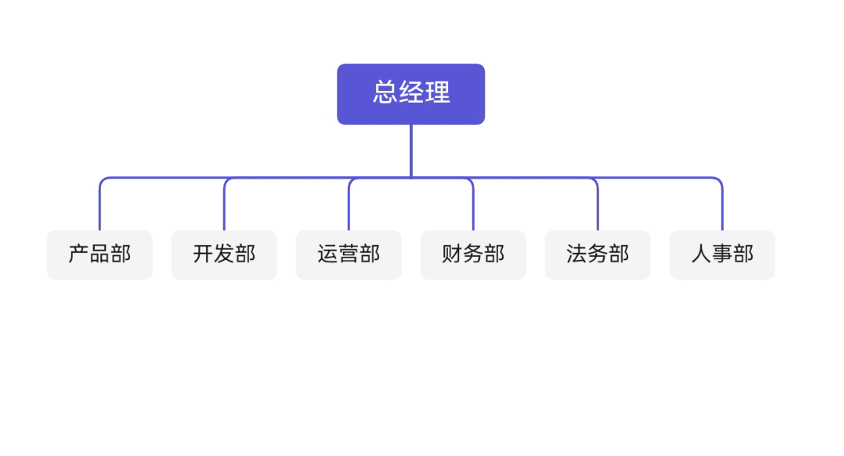
\includegraphics{Picture1.png}
	\caption{架构图}

\end{figure}
\subsection{各部门职责}
\begin{description}
	\item[总经理]根据董事会提出的战略目标,组织制定公司中产期发展战略与经营方案,并 推动实施;拟定公司内部管理构架的设置方案并签发公司的各类任命和调整;主持公司的全面经营管理工作,组织分解公司全年的工作任务;处理公司重大突发事 件和重大对外关系; 推进公司各类文化的建设,制度的推行,树立良好的企业形 象;召集、主持总经理办 公会议,总结工作,听取汇报,检查工作,督促进度和 协调矛盾
	\item[产品部]负责产品的需求方案的提出及运营策略的可行性建议;负责产品的内容规划; 统计网站各项数据和用户反馈,分析用户需求、行为,搜集产品运营中产生的产 品购买及网站功能需求,综合各部门的意见和建议,统筹安排,讨论、修改,制订出可行性方案;和开 发部、运营部等部门紧密结合,确保产品实现进度和质量,协调相关部门进行相关产品的开发及日常的维护。
	\item[开发部]根据产品部提出的互联网产品的原型,进行需求分析,系统设计,软件研发, 集成测试,安装部署以及运营维护工作。实现产品高效率、高用户体验以及高安 全性;负责 公司所有的互联网产品的运行维护工作,对各部门提出的产品升级和 错误修订需求,做出快速反应。
	\item[运营部]制定灼见的线上推广规范;坚持日常推广,维护搜索引擎后台,保证产品下 载量;进行网络调研和产品分析,将调研和分析结果反馈给上级,并进行持续跟 踪了解;灼见线上活动的组织、执行、总结、反馈和改进,不断拓展和丰富活动 内容;对产品新闻、排版和客户反馈的意见进行及时处理,不断扩大规模,实现 年度盈利目标;公司网络资源和网络媒体的整合,公司各项业务的网络和工作支撑。
	\item[财务部]根据公司经营目标,修订并实施财务制度、财务预算、财务日常核算、财务管理工作;执行财务计划,完成公司财务目标;编制及组织实施财务预算报告,月、季、年度财务报告;负责公司资金、资产管理工作。
	\item[法务部]参与集团重大经济活动的谈判工作,提出减少或避免法律风险的措施和法律 意见;审查、修改、会签经济合同、协议,协助和督促集团对重大经济合同、协议的履行;修订和完善合同管理制度,指导下属公司及其他业务部门制订合同管 理实施办法;制订公司自用合同的格式文本;会同相关部门对重大、重要合同进行 评审并出具审查意见;监督、检查各部门合同签订、履行、管理情况;参与合同纠 纷的调查处理,制定解决方案。
	\item[人事部]根据公司经营管理需要,设计各部门组织机构及人员编制;根据公司的人事方针与政策,制定部门业务工作的政策、程序和各项规章制度;负责计划与实施 员工招聘工作;根据公司经营管理的方针策略,负责计划、组织、检查及督促各项培训工作。
\end{description}
\section{营销策略}
\subsection{营销综述}
\subsubsection{核心——用户粘度}
“粘度”是衡量用户忠诚度计划的重要指标,一个用户的粘度越高就代表该用 户对所享受的产品或者服务的忠诚度越高,反之则越低。根据营销理论中的“28” 原则(即百分之二十的客户,完成了百分之八十的营业额或利润。)我们可以合 理推断出某种意义上回头客比新客对企业的贡献更大,同时在虚拟社区和电子商 务领域中更受关注的是用户粘度。因此如何切实有效的提升网民的用户粘度是本 公司营销策略的核心思想。
\subsubsection{定位——挑战与补缺}
综合前部分市场分析、竞争者分析以及战略蓝图的描述,我们可以初步明确自身的定位——挑战者及补缺者。

作为挑战者,我们不仅面临现有人才管理平台的实力竞争,还要面对原有传统社区服务模式的抗争。我们拥有的是以跨公司跨平台为主题的人才管理、更加便利的人才招聘等服务,倡导的是一种基于人员流动展开的全方位多角度的一站式服务。

作为补缺者,现在的垂直社区电商领域来说是一个空白市场,或者说是一个该领域企业提供的服务模式没有完全满足用户需求的细分市场,所以我们的服务可以有效填补这块服务模式有缺位的市场。
\subsection{推广策略}
\subsubsection{线上推广}
\paragraph{建立微信公众号}


微信早已是人们进行社交,信息获取的最主要的渠道,其影响力可见一斑, 尤其是那些提供广大用户需要信息的公众号。基于此大背景下,本公司为了更有 效地进行产品推广,将打造一个提供用户关于人才管理相关的信息平台,所提供的信息例如:
\begin{enumerate}[1)]
	\item 提供平台使用教程
	\item 人才培养类型推文
\end{enumerate}

\paragraph{搜索引擎推广}


投放广告到百度等平台。目前,百度、知乎等平台在用户生活中起到的作用是显而易见的,我们公司基于这一要素计划,制作一部有趣、富有特色以及具有吸引力的宣传视频以及一些软文,使得用户在搜索相关产品时可以第一时间看见本产品。
\paragraph{在各平台发布消息和软文,树立口碑}


雇佣一些人为产品造势,在微博、小红书、哔哩哔哩、抖音、贴吧、天涯等 平台传播产品用户体验,同时在一些高影响力的 UGC 社区如微博知乎豆瓣上 写软文,让更多的人知道万品客的优质便捷,同时这种口口相传的形式可以树立公司良好的形象,打造高质量的口碑
\subsubsection{线下推广}
线下的推广对于本产品来说更多的是辅助性作用,以提高品牌知名度为主。可以采取在各大路口投放LED屏广告、公交车站牌广告等形式。
\subsection{品牌策略}
\subsubsection{4C理论下的营销策略}
\begin{figure}[H]
	\centering
	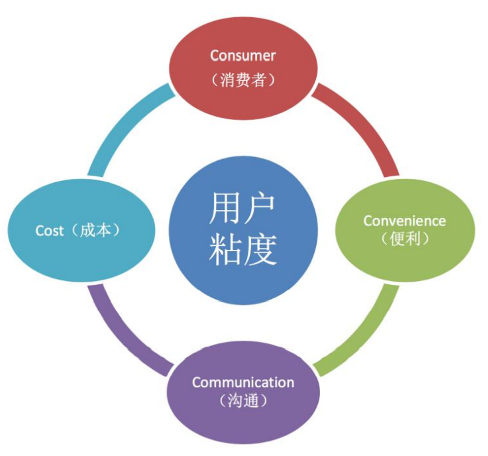
\includegraphics{marketing}
	\caption{4C理论下的营销策略图}
\end{figure}
\begin{description}
	\item [Customer 消费者]
	      企业首先要了解消费者的需求,根据用户的需求来提高产品。同时企业提供 的不仅仅是产品和服务,更重要的是由此产品的客户价值。如下文所示:
	      \begin{itemize}
		      \item 顾客需求:崇尚人性化、安全的服务,渴望更全面、更精细的服务,追求便 捷性。
		      \item 产品服务提供:更具个性化、便利性的万品客,基于人才招聘管理展开的一站式服务。
		      \item 相对应的客户价值:更具个性化、人性化的服务,更加便捷全面的服务,更 能调动用户参与度的服务,更高的用户体验。
	      \end{itemize}
	\item[Cost 成本]
		成本不仅包括顾客的货币支出,也包括顾客为此消耗的时间,体力和精力消 耗以及购买风险。如下文所示:
		\begin{itemize}
			\item 货币支出:(会员费)月费6元/月,年费66元/年
			\item 体力支出:全方位多角度的服务平台,方便快捷的操作体验Web服务端
			\item 购买风险:24h客户移动网络的服务
			\item 精力支出:包含有关人才招聘管理的各方面信息、拥有个性化定制服务
			\item 时间支出:一站式的服务、快捷全面的服务流程
		\end{itemize}
		\item[Convenience 便利]4C 营销理论强调企业在制定分销策略时,要更多的考虑顾客的方便,而不 是企业自己的方便。要通过好的售前,售中和售后服务来让顾客在购物的同时, 也享受到了便利。
		\begin{enumerate}[1)]
			\item 售前——让顾客及时获取相关信息并享受方便高效的服务 \\Web浏览器:及时提供关于人才招聘管理的最新相关资讯,最基本的客服咨询
			      \\微信公众号:发布一些关于人才招聘管理的推文咨询,最基本的客服咨询
			\item 售中——为顾客提供高价值的付费服务以及便捷的信息服务 \\会员专享去除广告,会员专享客服专线,VIP客户在线咨询,会员享受24时智能推送服务
			\item 售后——竭力为打造公司与客户之间的良好关系做基础
			      \\客服咨询:非会员16小时客服热线,会员独有客服专线
			      \\客服反馈:接受用户指出平台的BUG反馈,接受用户举报其他用户的违规 行为的投诉
			      \\客服建议:对顾客提出的优化产品设计以及服务改进的建议作出回应并感 谢,接受顾客提出的增加新功能的建议
		\end{enumerate}
	\item [Communication 沟通]
	      企业应通过同顾客进行积极有效的双向沟通,建立基于共同利益的新型企业 /顾客关系。双向沟通可以通过提高用户参与度提高用户粘性,进而为打造良好 客户关系奠定基础。
	      \begin{description}
		      \item[载体——多角度与顾客进行沟通]
			      我们采取多渠道多方位的方式与顾客进行频繁紧密的沟通,不仅能将公司最 新的信息提供给客户同时也能及时针对用户对公司提出的反馈做出回应,从而让用户完全的感受到我们对其贴心周到的服务。\\用户进行反馈时,都是与客服进行间接或者直接的沟通,客服所提供服务质 量的好坏直接影响着他们对本公司的印象以及用户的体验和心情,为了塑造良好 的企业形象同时也为了更好的解决顾客所提出的较专业的或者较情绪化方面的我们公司的客服经过严格培训后方可上岗,他们将及时高效解决用户的各种其他问题。
		      \item[机制——和谐沟通 ]
			      我们将以“做到无阻力沟通——及时反馈——回访顾客——做出激励”的方 式作出最完善的沟通机制。我们将竭力做到使用户与公司之间无阻力沟通,清除 一切阻挡双向沟通的障碍;若用户提出意见,我们将会及时作出反馈,最大化减 少用户等待回应的时间;当问题解决之后需要回访顾客,使用户感到被尊重,塑 造一个良好的企业形象;同时对于经常反馈意见的顾客,我们还会采取奖励的方 式回馈用户,以此激励顾客继续提出建议。
		      \item[其他活动——对用户的促销活动]
			      为进一步打造用户与公司之间的良好关系并提高他们的积极性,我们将推出以下活动:
			      \begin{itemize}
				      \item 送代金劵来更好地回馈我们的消费者,每一年都会选出符合相关标准的 会员,免费赠送一定金额的代金劵。努力通过这个过程增加用户积极性,提供更 有质量的生活。
				      \item 送代金劵来更好地回馈我们的消费者,每一年都会选出符合相关标准的 会员,免费赠送一定金额的代金劵。努力通过这个过程增加用户积极性,提供更 有质量的生活。
			      \end{itemize}
	      \end{description}
\end{description}
\subsubsection{会员制度}
我们将采用会员制度,划分3个月/半年/一年/终身会员等时间期限。

会员可以享用更多的特权功能,在使用平台招聘人才等功能中可以进行定制筛选,对于人才也会有优先推荐权。

另外每一位会员都会配备有VIP客服,提升会员的售后反馈服务体验。
\subsubsection{深度服务}
对于有特殊需求的企业,我们可以在提供原始平台的基础上提供定制化服务。

基于SaaS的商业模式,我们将致力于为企业提供更好更贴切的服务体验,解决企业在人才管理方面的问题,助力企业更好地管理员工,提升经济效益。

\begin{enumerate}[1)]
	\item 本平台会选派专业人员进入到企业内部,深入客户的业务领域,诊断其办公过程中的需求痛点、难点,根据测评结果反馈平台产品,优化管理系统,分享成功案例。
	\item 提供产品使用能力的培训与教学服务,提供本产品各项功能以及完成某一确定需求的教学视频,助力各大HR更好地实现办公。
	\item 深入诊断客户的使用性问题,根据对方给出的特定需要,提供技术支持与服务咨询,定制出个性化解决方案供专人专用。
	\item 通过一系列定制化服务,让本产品能更好地贴合各行各业,同时提升客户使用的便利性,增加客户使用依赖。

\end{enumerate}
\section{风险分析}
\subsection{风险预测}
\subsubsection{市场风险}
\paragraph{本项目创立阶段初期,可能会遭遇下列某项或多项市场风险:}
\begin{itemize}
	\item [1)]
	      该线上HR系统开设立意较为新颖,各大公司对于该项目的认知程度低,在投入运行初期可能会存在顾客量少于预期,达不到营销目标所要求的知名度。并且有可能会陷入顾客少——知名度降低相互作用的恶循环之中。

	\item [2)]
	      虽然线上HR系统是新型行业,但对于互联网公司来说,这方面一定有所涉猎,如果有公司入场,市场竞争激烈,使项目的市场增长率下降。

	\item [3)]
	      根据调查问卷调查,无论是在市中心工作的在职员工店员还是市中心周围游客、访客。因为对本项目熟知度不高,所以相比本项目提供的休息环境,多数人更偏向于去较大的商务酒店、旅馆进行休息。因此本项目并不能吸引预期数目的顾客,低于营销要求
\end{itemize}
\subsubsection{成本控制风险}
\paragraph{除市场外因带来的风险外,本项目在创建初期还会遇到涉及资金成本的风险:}
\begin{itemize}

	\item[1)]宣传对象:根据需求量调查,本项目优先宣传为国企和事业单位时达到最优。但这些企业本身因需求量大,市场潜力巨大而成为各家各种项目争抢的地方,而且在设计到敏感的人事管理方面,其顾虑也往往比较多,难以形成稳定的客户来源,在设立初期就要考虑招揽客户的成本。


	\item[2)]服务器设置:如果设置在二线三线城市,则地价租金相对较少,而且招工工资也相对便宜,但是一线城市的客户的访问延时也会加大,与此同时,二三线城市的人才资源也相对稀缺。


	\item[3)]运营日常消费:为了维护服务器的正常运行,需要经常更换冗余硬件,并安排专人进行运维维护


	\item[4)]雇员工资问题:需要招募员工,对整个网络以及服务器系统进行维护和升级。在创业初期,当营业额并不乐观时,雇员的薪酬问题会给该项目带来较大的压力。而项目组还要平衡人力投入与收益回报之间的平衡问题。
\end{itemize}
\subsubsection{管理风险}
\begin{itemize}
	\item[1)]面对群众方面:本项目的面对是对人事管理有进阶需求的企业,需要考虑各个公司对审视管理的不同需求和想法。对于每位客户,需要保证在最大限度确保他们需求的功能和特性的前提下保证对该项目的合法合理使用。

	\item[2)]店员方面:在创业初期无论运营者还是雇员,对该项工作的实际操作都不会马上熟练。参与该项目的成员相对来说,缺乏对于店面的管理经验以及科学决策能力,不能对市场和管理具有良好的认知和实践。在实际运营中会存在失误而导致与顾客之间产生的各种矛盾冲突
\end{itemize}
\subsubsection{技术风险}
本项目尚处于创业的初级阶段,在服务提供和市场要求等方面还未达到完美的结合。同时在创业起始时,项目店内设施设备(例如电脑等)相对未完备,而因为无法短时间内找到物美价廉的替代品而导致一定的技术风险。
\subsection{风险控制}
\begin{itemize}
	\item[1)]针对达不到营销目标所存在的风险,项目应将广告等促销宣传活动做到位,以此来缩短消费者对本项目的认知周期。


	\item[2)]发展特色服务,在新颖的功能优势上更进一步。采取各种营销手段,树立良好的品牌形象,以此在消费者中形成良好的口碑效应。


	\item[3)]建立和完善市场信息反馈体系,定期安排员工以纸面或网上问卷的方式对消费者进行市场调查,通过调查结果及时把握市场变动趋势,把握消费者的喜好倾向。
\end{itemize}
\subsubsection{发展新项目的独特之处}
\begin{itemize}
	\item[1)]参与保险:在创业初期签署可靠的若干商业保险,避免当一旦项目失败,保险项目将承担部分损失。
	\item[2)]吸收风险投资:风险项目主要参与风险损失和风险收益的分摊。
\end{itemize}
\subsubsection{技术创新风险的财务转移}

在项目的前期阶段,项目组应该搜索整理相关职业在市场中的发展趋势,以此为参考,对本项目未来的竞争环节做出比较准确预见和判断,对成本进行相关预测,以此提高对不确定性因素的免疫力。加上对成本控制考核机制的改善,能够降低成本转嫁行为对企业的危害。
\subsubsection{加强对成本的规划与预测}
本项目会建立各项制度,严格确定用人标准,加强管理。在管理层方面,管理人员要具有服务精神和奉献精神,要多学习管理方法和管理经验。
\section{财务分析}
\subsection{财务状况}
做本项目系统,在前期的开发成本上需要有巨大支出,根据现有情况做出的关于企业的前期开支和日常开支的表格如下:
\begin{table}[H]
	\centering
	\begin{tabular}{|l|l|l|}
		\hline
		前期开支 & 公司成立和注册 & 10万       \\ \hline
		         & 购买设备       & 20万       \\ \hline
		         & 开发费用       & 285万      \\ \hline
		         & 系统测试       & 15万       \\ \hline
		日常开支 & 维修费用       & 10万       \\ \hline
		         & 员工工资       & 5000/人/月 \\ \hline
		         & 其他费用       & 2500/月    \\ \hline
	\end{tabular}
\end{table}
\subsection{会计报表}
\subsubsection{资产负债表}
\begin{table}[H]
	\centering
	\begin{tabular}{|l|l|l|l|l|l|}
		\hline
		年份                 & 第一年 & 第二年 & 第三年  & 第四年  & 第五年 \\ \hline
		流动资产:           &        &        &         &         &        \\ \hline
		货币资金             & 102    & 597.5  & 1357    & 1762    & 2249   \\ \hline
		应收账款             & 422    & 1048   & 1329.25 & 1368.25 & 1056   \\ \hline
		减:坏账准备         & 2      & 5      & 6       & 8       & 9      \\ \hline
		应收坏账净额         & 420    & 1043   & 1323.25 & 1360.25 & 1047   \\ \hline
		存货                 & 119    & 100    & 110     & 120     & 127    \\ \hline
		待摊费用             & 22     & 16     & 32      & 22      & 11     \\ \hline

		固定资产:           &        &        &         &         &        \\ \hline
		固定资产原值         & 136    & 135    & 272     & 272     & 272    \\ \hline
		减:累计折旧         & 16     & 32     & 48      & 64      & 80     \\ \hline
		固定资产净值         & 120    & 103    & 224     & 208     & 192    \\ \hline
		无形资产             & 240    & 210    & 180     & 150     & 120    \\ \hline
		资产合计             & 1023   & 2069.5 & 3226.25 & 3622.25 & 3746   \\ \hline

		流动负债             &        &        &         &         &        \\ \hline
		应付账款             & 28     & 73     & 250     & 270     & 300    \\ \hline
		短期借款             & 0      & 224    & 0       & 0       & 0      \\ \hline
		                     & 28     & 297    & 250     & 270     & 300    \\ \hline
		长期借款             & 212    &        & 0       & 0       & 0      \\ \hline
		负债合计             & 240    & 297    & 250     & 270     & 300    \\ \hline

		所有者权益           &        &        &         &         &        \\ \hline
		实收资本             & 800    & 800    & 800     & 800     & 800    \\ \hline
		盈余公积             & 0      & 113    & 320     & 420     & 420    \\ \hline
		未分配利润           & -17    & 859.5  & 1856.25 & 2132.25 & 2226   \\ \hline
		所有者权益合计       & 783    & 1772.5 & 2976.25 & 3352.25 & 3446   \\ \hline

		负债和所有者权益合计 & 1023   & 2069.5 & 3226.25 & 3622.25 & 3746   \\ \hline
	\end{tabular}
\end{table}
\subsubsection{利润表}
\begin{table}[H]
	\centering
	\begin{tabular}{|l|l|l|l|l|l|}
		\hline
		年份                 & 第一年 & 第二年 & 第三年  & 第四年  & 第五年 \\ \hline
		一、主营业务收入     & 1406   & 3496   & 4653    & 5511    & 5986   \\ \hline
		减:主营业务成本     & 212    & 441    & 666     & 845     & 982    \\ \hline
		减:主营业税金及附加 & 24     & 60     & 80      & 94      & 102    \\ \hline
		二、主营业务利润     & 1170   & 2995   & 3907    & 4572    & 4902   \\ \hline
		加:其他业务利润     & 0      & 0      & 0       & 0       & 0      \\ \hline
		减:营业费用         & 870    & 1623   & 1130    & 1331    & 1410   \\ \hline
		减:管理费用         & 295    & 204    & 278     & 374     & 500    \\ \hline
		减:财务费用         & 12     & 12     & 12      & 12      & 12     \\ \hline
		                     &        &        &         &         &        \\ \hline
		三、营业利润         & -7     & 1156   & 2487    & 2855    & 2980   \\ \hline
		加:投资收益         & 0      & 0      & 0       & 0       & 0      \\ \hline
		加:营业外收入       & 0      & 0      & 0       & 0       & 0      \\ \hline
		减:营业外支出       & 10     & 10     & 12      & 12      & 12     \\ \hline
		四、利润总额         & -17    & 1146   & 2475    & 2843    & 2968   \\ \hline
		减:所得税           & 0      & 286.5  & 618.75  & 710.75  & 742    \\ \hline
		五:净利润           & -17    & 859.5  & 1856.25 & 2132.25 & 2226   \\ \hline
	\end{tabular}
\end{table}
\subsection{财务分析}
\subsubsection{偿债能力分析}
\begin{table}[H]
	\centering
	\begin{tabular}{|l|l|l|l|l|l|}
		\hline
		年份         & 第一年      & 第二年      & 第三年     & 第四年      & 第五年      \\ \hline
		流动比率     & 23.67857143 & 5.914141414 & 11.289     & 12.08981481 & 11.44666667 \\ \hline
		速动比率     & 18.64285714 & 5.523569024 & 10.721     & 11.56388889 & 10.98666667 \\ \hline
		资产负债率   & 23.46\%     & 14.35\%     & 7.75\%     & 7.45\%      & 8.01\%      \\ \hline
		股东权益比率 & 76.54\%     & 85.65\%     & 92.25\%    & 92.55\%     & 91.99\%     \\ \hline
		产权比率     & 0.30651341  & 0.167559944 & 0.08399832 & 0.080542919 & 0.087057458 \\ \hline
	\end{tabular}
\end{table}
评价偿债能力的财务比率主要有流动比率、速动比率、资产负债率、股东权益比率、产权比率等,未来五年的速动比率符合速动比例为1时的要求,一般认为速动比率越高偿债能力越强;资产负债率是反映企业的综合偿债能力,资产负债率越高,企业的偿还债务的能力越差。根据上表分析可知,企业未来五年的资产负债率除了前两年的企业创建初的波动之外,基本满足在7\%—8\%之间波动,表明我们企业的偿债能力越来越强,且趋于稳定。
\subsubsection{盈利能力分析}
\begin{table}[H]
	\centering
	\begin{tabular}{|l|l|l|l|l|l|}
		\hline
		年份       & 第一年  & 第二年  & 第三年  & 第四年  & 第五年  \\ \hline
		资产净利率 & -1.66\% & 41.53\% & 57.54\% & 58.87\% & 59.42\% \\ \hline
		销售毛利率 & 83.21\% & 85.67\% & 83.97\% & 82.96\% & 81.89\% \\ \hline
	\end{tabular}
\end{table}
评价企业的盈利能力可以使用资产净利率、销售毛利率。由表可以看出企业的资产净利率呈稳定上升的趋势,而销售毛利率在第二年达到高峰,随后下降,却一直稳定在80%以上,这表明企业的营业成本控制可能还需要加强,但是企业的经营效率稳定,反映出公司在经营的过程中保持一个良好的发展态势。较高的资产净利率和不错的销售毛利率,表明公司资本回报率较高,可以在经营一两年后开始盈利。并且资产净利率和销售毛利率都趋向稳定,也能反映出行业和经济环境对公司经营的影响不会太大。


由于初始资金330万。结合利润表中每年的利润率。
\begin{table}[H]
	\centering
	\begin{tabular}{|l|l|l|l|l|l|l|}
	\hline
		  & 成本费用 & 第一年  & 第二年   & 第三年     & 第四年     & 第五年  \\ \hline
	现金流   & 330  & -17  & 859.5 & 1856.25 & 2132.25 & 2226 \\ \hline
	累计现金流 &      & -347 & 512.5 & 2368.75 & 4501    & 6727 \\ \hline
	\end{tabular}
	\end{table}
	累计现金流在第二年的时候开始取正,预计公司在第三年的时候可以开始盈利。
\end{document}